\chapter{DX-038 - BlockLab Rename And Migration}\label{record-134}

\noindent{\footnotesize\color{BookMuted}\path{docs/design/DX-038-blocklab-rename-and-migration.md}\par}\smallskip

\begin{RecordMeta}
title: "DX-038 - BlockLab Rename And Migration"
legend: DX
lane: design
issue: https://github.com/flyingrobots/bijou/issues/271

\end{RecordMeta}

\section{Linked Issue}\label{record-134-linked-issue}

\begin{itemize}
\tightlist
\item
  https://github.com/flyingrobots/bijou/issues/271
\end{itemize}

\section{Sponsored Human}\label{record-134-sponsored-human}

A Bijou maintainer wants the story and component workbench to have a project-owned name that does not imply affiliation with the browser Storybook product, while keeping the existing workflow understandable for users who already know \texttt{n\allowbreak{}p\allowbreak{}m\allowbreak{} \allowbreak{}r\allowbreak{}u\allowbreak{}n\allowbreak{} \allowbreak{}s\allowbreak{}t\allowbreak{}o\allowbreak{}r\allowbreak{}y\allowbreak{}b\allowbreak{}o\allowbreak{}o\allowbreak{}k}.

\section{Sponsored Agent}\label{record-134-sponsored-agent}

An agent needs stable names for scripts, Blocks, command intents, surface ids, and docs links. It should not have to infer whether ``storybook'' means Bijou's terminal workbench, the external product, or a generic story-driven workflow.

\section{Hill}\label{record-134-hill}

Rename the current Storybook-labeled workstation to \textbf{BlockLab} across human visible surfaces and future-facing contracts, while preserving a short compatibility path for existing commands.

This is product hygiene, not a legal conclusion. The current name creates avoidable ambiguity because Storybook is an established external product. Bijou can keep story-driven component development while naming its own terminal-native surface differently.

\section{Current Truth}\label{record-134-current-truth}

The current repo exposes a story-driven workstation through:

\begin{itemize}
\tightlist
\item
  \texttt{n\allowbreak{}p\allowbreak{}m\allowbreak{} \allowbreak{}r\allowbreak{}u\allowbreak{}n\allowbreak{} \allowbreak{}s\allowbreak{}t\allowbreak{}o\allowbreak{}r\allowbreak{}y\allowbreak{}b\allowbreak{}o\allowbreak{}o\allowbreak{}k}
\item
  \texttt{n\allowbreak{}p\allowbreak{}m\allowbreak{} \allowbreak{}r\allowbreak{}u\allowbreak{}n\allowbreak{} \allowbreak{}s\allowbreak{}t\allowbreak{}o\allowbreak{}r\allowbreak{}y\allowbreak{}b\allowbreak{}o\allowbreak{}o\allowbreak{}k\allowbreak{}:\allowbreak{}i\allowbreak{}n\allowbreak{}d\allowbreak{}e\allowbreak{}x}
\item
  \texttt{n\allowbreak{}p\allowbreak{}m\allowbreak{} \allowbreak{}r\allowbreak{}u\allowbreak{}n\allowbreak{} \allowbreak{}d\allowbreak{}o\allowbreak{}g\allowbreak{}f\allowbreak{}o\allowbreak{}o\allowbreak{}d\allowbreak{}:\allowbreak{}s\allowbreak{}t\allowbreak{}o\allowbreak{}r\allowbreak{}y\allowbreak{}b\allowbreak{}o\allowbreak{}o\allowbreak{}k}
\item
  \texttt{e\allowbreak{}x\allowbreak{}a\allowbreak{}m\allowbreak{}p\allowbreak{}l\allowbreak{}e\allowbreak{}s\allowbreak{}/\allowbreak{}d\allowbreak{}o\allowbreak{}c\allowbreak{}s\allowbreak{}/\allowbreak{}s\allowbreak{}t\allowbreak{}o\allowbreak{}r\allowbreak{}y\allowbreak{}b\allowbreak{}o\allowbreak{}o\allowbreak{}k\allowbreak{}.\allowbreak{}t\allowbreak{}s}
\item
  \texttt{e\allowbreak{}x\allowbreak{}a\allowbreak{}m\allowbreak{}p\allowbreak{}l\allowbreak{}e\allowbreak{}s\allowbreak{}/\allowbreak{}d\allowbreak{}o\allowbreak{}c\allowbreak{}s\allowbreak{}/\allowbreak{}s\allowbreak{}t\allowbreak{}o\allowbreak{}r\allowbreak{}y\allowbreak{}b\allowbreak{}o\allowbreak{}o\allowbreak{}k\allowbreak{}-\allowbreak{}a\allowbreak{}p\allowbreak{}p\allowbreak{}.\allowbreak{}t\allowbreak{}s}
\item
  \texttt{e\allowbreak{}x\allowbreak{}a\allowbreak{}m\allowbreak{}p\allowbreak{}l\allowbreak{}e\allowbreak{}s\allowbreak{}/\allowbreak{}d\allowbreak{}o\allowbreak{}c\allowbreak{}s\allowbreak{}/\allowbreak{}s\allowbreak{}t\allowbreak{}o\allowbreak{}r\allowbreak{}y\allowbreak{}b\allowbreak{}o\allowbreak{}o\allowbreak{}k\allowbreak{}-\allowbreak{}w\allowbreak{}o\allowbreak{}r\allowbreak{}k\allowbreak{}s\allowbreak{}t\allowbreak{}a\allowbreak{}t\allowbreak{}i\allowbreak{}o\allowbreak{}n\allowbreak{}.\allowbreak{}t\allowbreak{}s}
\item
  visible labels such as \texttt{B\allowbreak{}i\allowbreak{}j\allowbreak{}o\allowbreak{}u\allowbreak{} \allowbreak{}S\allowbreak{}t\allowbreak{}o\allowbreak{}r\allowbreak{}y\allowbreak{}b\allowbreak{}o\allowbreak{}o\allowbreak{}k}, \texttt{S\allowbreak{}t\allowbreak{}o\allowbreak{}r\allowbreak{}y\allowbreak{}b\allowbreak{}o\allowbreak{}o\allowbreak{}k}, and \texttt{S\allowbreak{}t\allowbreak{}o\allowbreak{}r\allowbreak{}y\allowbreak{}b\allowbreak{}o\allowbreak{}o\allowbreak{}k\allowbreak{} \allowbreak{}W\allowbreak{}o\allowbreak{}r\allowbreak{}k\allowbreak{}s\allowbreak{}t\allowbreak{}a\allowbreak{}t\allowbreak{}i\allowbreak{}o\allowbreak{}n}
\item
  DOGFOOD Block and registry names such as \texttt{S\allowbreak{}t\allowbreak{}o\allowbreak{}r\allowbreak{}y\allowbreak{}b\allowbreak{}o\allowbreak{}o\allowbreak{}k\allowbreak{}W\allowbreak{}o\allowbreak{}r\allowbreak{}k\allowbreak{}b\allowbreak{}e\allowbreak{}n\allowbreak{}c\allowbreak{}h\allowbreak{}B\allowbreak{}l\allowbreak{}o\allowbreak{}c\allowbreak{}k}
\item
  docs that describe a ``Storybook-style'' workbench
\end{itemize}

The product shape is already useful: it has a story catalog, variants, profile presets, structured docs fields, matrix capture, AppFrame integration, and a text-first index. The naming layer is the weak part.

\section{Name Decision}\label{record-134-name-decision}

Use \textbf{BlockLab} as the product name.

Proposed vocabulary:

\begin{center}
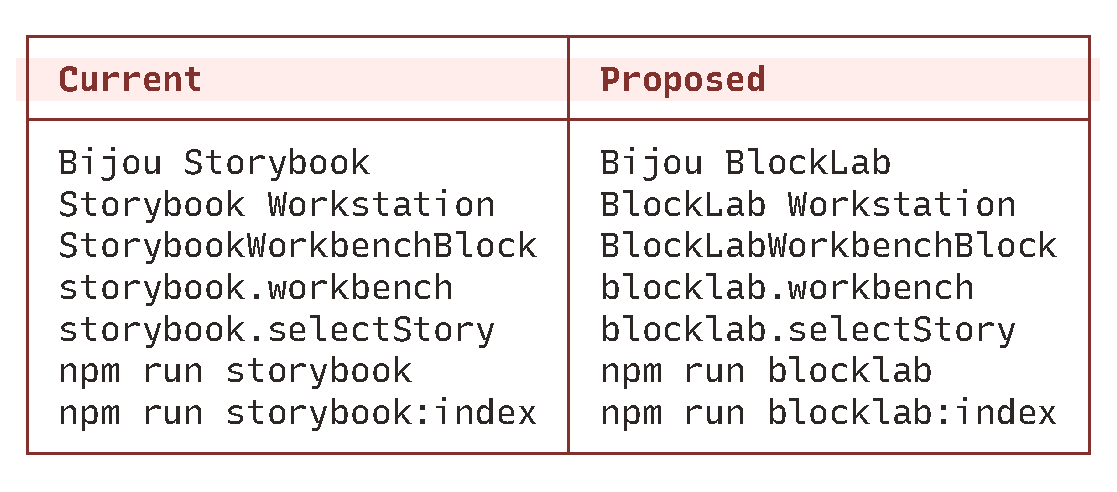
\includegraphics[width=\linewidth]{figures/tables/table-033-g1-1.pdf}
\par\smallskip{\scriptsize\color{BookMuted}Rows 1–7. Actual Bijou table component.}
\end{center}


Compatibility aliases should remain for one migration window:

\begin{CodeBlock}
npm run storybook
npm run storybook:index
npm run dogfood:storybook
\end{CodeBlock}

Those aliases should call the BlockLab entrypoints and may print a concise deprecation note if the runtime can do so without polluting deterministic index output.

\section{TUI Mockup}\label{record-134-tui-mockup}

Wide terminal:

\begin{CodeBlock}
Bijou BlockLab | notification-system | Live stack | Rich
+ catalog -------------------++ preview ---------------------------++ lab -----------------------+
| 72 stories                  || notification-system                || Selection                  |
| > notification-system       || + Live stack --------------------+ || story=notification-system  |
|   framed-shell              || | release dashboard              | || variant=live-stack        |
|   command-palette           || | Canaries stable in eu-west     | || profile=interactive       |
|   table-responsive          || +-------------------------------+ ||                              |
|                             || Docs                              || Required modes             |
| Families                    || Use when                          || interactive: ready         |
| Feedback overlays           || - surface owns transient state     || static: ready              |
| Navigation                  || - lower modes preserve message     || pipe: ready                |
| Blocks                      ||                                   || accessible: ready          |
+-----------------------------++-----------------------------------++-----------------------------+
q quit | / search | g globals | c controls | a actions | t tests | ,/. variant | 1-4 profile
\end{CodeBlock}

Narrow terminal:

\begin{CodeBlock}
Bijou BlockLab
notification-system

+ Live stack --------------------+
| release dashboard              |
| Canaries stable in eu-west     |
+-------------------------------+

Profile: Rich / interactive / 60 cols
Variant: live-stack
Modes: interactive static pipe accessible

Tabs: preview docs controls tests actions
\end{CodeBlock}

\section{Lower Modes}\label{record-134-lower-modes}

Pipe mode should remain deterministic and artifact-friendly:

\begin{CodeBlock}
blocklab index
stories=72
families=31
variants=144
requiredModes=interactive,static,pipe,accessible

family Feedback overlays and history
- notification-system | package=bijou-tui | variants=live-stack,history-review,framed-routing
\end{CodeBlock}

Accessible mode should describe purpose and state instead of chrome:

\begin{CodeBlock}
BlockLab workbench. Story notification-system. Variant Live stack.
Profile Rich. Required modes are all ready. Source examples/notifications/main.ts.
Preview summary: release dashboard, canaries stable in eu-west.
\end{CodeBlock}

\section{Accessibility / Assistive Posture}\label{record-134-accessibility-assistive-posture}

The rename must not make the workbench more visual-only. Every renamed surface keeps existing lower-mode facts:

\begin{itemize}
\tightlist
\item
  story id
\item
  story title
\item
  package
\item
  source path
\item
  selected variant
\item
  selected profile
\item
  required mode coverage
\item
  capture matrix status
\end{itemize}

Future \texttt{B\allowbreak{}l\allowbreak{}o\allowbreak{}c\allowbreak{}k\allowbreak{}L\allowbreak{}a\allowbreak{}b} labels should be localizable visible text. Machine tokens such as command ids and event discriminants can use \texttt{b\allowbreak{}l\allowbreak{}o\allowbreak{}c\allowbreak{}k\allowbreak{}l\allowbreak{}a\allowbreak{}b\allowbreak{}.\allowbreak{}*} but should not be translated.

\section{Localization / Directionality Posture}\label{record-134-localization-directionality-posture}

New visible strings must enter \texttt{e\allowbreak{}x\allowbreak{}a\allowbreak{}m\allowbreak{}p\allowbreak{}l\allowbreak{}e\allowbreak{}s\allowbreak{}/\allowbreak{}d\allowbreak{}o\allowbreak{}c\allowbreak{}s\allowbreak{}/\allowbreak{}i\allowbreak{}1\allowbreak{}8\allowbreak{}n\allowbreak{}/\allowbreak{}s\allowbreak{}o\allowbreak{}u\allowbreak{}r\allowbreak{}c\allowbreak{}e\allowbreak{}/\allowbreak{}d\allowbreak{}o\allowbreak{}g\allowbreak{}f\allowbreak{}o\allowbreak{}o\allowbreak{}d\allowbreak{}-\allowbreak{}s\allowbreak{}t\allowbreak{}r\allowbreak{}i\allowbreak{}n\allowbreak{}g\allowbreak{}s\allowbreak{}.\allowbreak{}c\allowbreak{}s\allowbreak{}v} with \texttt{e\allowbreak{}n}, \texttt{f\allowbreak{}r}, \texttt{e\allowbreak{}s}, and \texttt{d\allowbreak{}e} rows. The rename should update generated catalog files in the same PR, and \texttt{n\allowbreak{}p\allowbreak{}m\allowbreak{} \allowbreak{}r\allowbreak{}u\allowbreak{}n\allowbreak{} \allowbreak{}d\allowbreak{}o\allowbreak{}g\allowbreak{}f\allowbreak{}o\allowbreak{}o\allowbreak{}d\allowbreak{}:\allowbreak{}i\allowbreak{}1\allowbreak{}8\allowbreak{}n\allowbreak{}:\allowbreak{}c\allowbreak{}o\allowbreak{}m\allowbreak{}p\allowbreak{}l\allowbreak{}e\allowbreak{}t\allowbreak{}e} should be run against the branch.

Directionality does not change for this rename. The UI must continue to route localized copy through DOGFOOD's localization port rather than hard-coded view helpers.

\section{Agent Inspectability / Explainability Posture}\label{record-134-agent-inspectability-explainability-posture}

Agents should be able to tell that \texttt{B\allowbreak{}l\allowbreak{}o\allowbreak{}c\allowbreak{}k\allowbreak{}L\allowbreak{}a\allowbreak{}b} is the canonical surface without scraping UI strings. The rename should update:

\begin{itemize}
\tightlist
\item
  Block metadata names and tags
\item
  surface inventory ids and descriptions
\item
  command intents
\item
  story matrix report titles
\item
  deterministic index title
\item
  docs references
\end{itemize}

The compatibility aliases should be treated as command-level affordances, not as canonical product names.

\section{Linked Invariants}\label{record-134-linked-invariants}

\begin{itemize}
\tightlist
\item
  GitHub Issues are the live tracker; this design is linked to \#271.
\item
  DOGFOOD localization completeness gates protect new visible strings.
\item
  Blocks own product semantics; components remain leaf rendering vocabulary.
\item
  Text-first outputs stay deterministic for CI, agents, and fixtures.
\end{itemize}

\section{Migration Plan}\label{record-134-migration-plan}

\begin{enumerate}
\def\labelenumi{\arabic{enumi}.}
\tightlist
\item
  Introduce BlockLab docs language and visible product labels.
\item
  Add \texttt{b\allowbreak{}l\allowbreak{}o\allowbreak{}c\allowbreak{}k\allowbreak{}l\allowbreak{}a\allowbreak{}b} and \texttt{b\allowbreak{}l\allowbreak{}o\allowbreak{}c\allowbreak{}k\allowbreak{}l\allowbreak{}a\allowbreak{}b\allowbreak{}:\allowbreak{}i\allowbreak{}n\allowbreak{}d\allowbreak{}e\allowbreak{}x} scripts.
\item
  Keep \texttt{s\allowbreak{}t\allowbreak{}o\allowbreak{}r\allowbreak{}y\allowbreak{}b\allowbreak{}o\allowbreak{}o\allowbreak{}k}, \texttt{s\allowbreak{}t\allowbreak{}o\allowbreak{}r\allowbreak{}y\allowbreak{}b\allowbreak{}o\allowbreak{}o\allowbreak{}k\allowbreak{}:\allowbreak{}i\allowbreak{}n\allowbreak{}d\allowbreak{}e\allowbreak{}x}, and \texttt{d\allowbreak{}o\allowbreak{}g\allowbreak{}f\allowbreak{}o\allowbreak{}o\allowbreak{}d\allowbreak{}:\allowbreak{}s\allowbreak{}t\allowbreak{}o\allowbreak{}r\allowbreak{}y\allowbreak{}b\allowbreak{}o\allowbreak{}o\allowbreak{}k} as compatibility aliases for one migration window.
\item
  Rename user-visible AppFrame page title and settings label.
\item
  Rename DOGFOOD Block contracts and registry entries from \texttt{S\allowbreak{}t\allowbreak{}o\allowbreak{}r\allowbreak{}y\allowbreak{}b\allowbreak{}o\allowbreak{}o\allowbreak{}k\allowbreak{}W\allowbreak{}o\allowbreak{}r\allowbreak{}k\allowbreak{}b\allowbreak{}e\allowbreak{}n\allowbreak{}c\allowbreak{}h\allowbreak{}B\allowbreak{}l\allowbreak{}o\allowbreak{}c\allowbreak{}k} to \texttt{B\allowbreak{}l\allowbreak{}o\allowbreak{}c\allowbreak{}k\allowbreak{}L\allowbreak{}a\allowbreak{}b\allowbreak{}W\allowbreak{}o\allowbreak{}r\allowbreak{}k\allowbreak{}b\allowbreak{}e\allowbreak{}n\allowbreak{}c\allowbreak{}h\allowbreak{}B\allowbreak{}l\allowbreak{}o\allowbreak{}c\allowbreak{}k}.
\item
  Rename command intents and surface ids from \texttt{s\allowbreak{}t\allowbreak{}o\allowbreak{}r\allowbreak{}y\allowbreak{}b\allowbreak{}o\allowbreak{}o\allowbreak{}k\allowbreak{}.\allowbreak{}*} to \texttt{b\allowbreak{}l\allowbreak{}o\allowbreak{}c\allowbreak{}k\allowbreak{}l\allowbreak{}a\allowbreak{}b\allowbreak{}.\allowbreak{}*}.
\item
  Update localization rows and generated catalogs.
\item
  Update docs, tests, and teardown command tables.
\end{enumerate}

\section{Tests To Write First}\label{record-134-tests-to-write-first}

\begin{itemize}
\tightlist
\item
  A focused rename test that expects the default title to be \texttt{B\allowbreak{}i\allowbreak{}j\allowbreak{}o\allowbreak{}u\allowbreak{} \allowbreak{}B\allowbreak{}l\allowbreak{}o\allowbreak{}c\allowbreak{}k\allowbreak{}L\allowbreak{}a\allowbreak{}b}.
\item
  A framed AppFrame test that expects the page title \texttt{B\allowbreak{}l\allowbreak{}o\allowbreak{}c\allowbreak{}k\allowbreak{}L\allowbreak{}a\allowbreak{}b}.
\item
  A DOGFOOD settings test that expects \texttt{B\allowbreak{}l\allowbreak{}o\allowbreak{}c\allowbreak{}k\allowbreak{}L\allowbreak{}a\allowbreak{}b\allowbreak{} \allowbreak{}W\allowbreak{}o\allowbreak{}r\allowbreak{}k\allowbreak{}s\allowbreak{}t\allowbreak{}a\allowbreak{}t\allowbreak{}i\allowbreak{}o\allowbreak{}n}.
\item
  A Block metadata test that expects \texttt{B\allowbreak{}l\allowbreak{}o\allowbreak{}c\allowbreak{}k\allowbreak{}L\allowbreak{}a\allowbreak{}b\allowbreak{}W\allowbreak{}o\allowbreak{}r\allowbreak{}k\allowbreak{}b\allowbreak{}e\allowbreak{}n\allowbreak{}c\allowbreak{}h\allowbreak{}B\allowbreak{}l\allowbreak{}o\allowbreak{}c\allowbreak{}k}.
\item
  A script-registration test proving \texttt{b\allowbreak{}l\allowbreak{}o\allowbreak{}c\allowbreak{}k\allowbreak{}l\allowbreak{}a\allowbreak{}b} and \texttt{b\allowbreak{}l\allowbreak{}o\allowbreak{}c\allowbreak{}k\allowbreak{}l\allowbreak{}a\allowbreak{}b\allowbreak{}:\allowbreak{}i\allowbreak{}n\allowbreak{}d\allowbreak{}e\allowbreak{}x} exist and legacy scripts still resolve.
\item
  An i18n completeness run proving every changed visible string has supported locale rows.
\end{itemize}

\section{Non-Goals}\label{record-134-non-goals}

\begin{itemize}
\tightlist
\item
  No direct Storybook compatibility layer.
\item
  No browser runtime.
\item
  No package rename outside the workbench surface.
\item
  No claim about trademark law.
\item
  No removal of compatibility scripts in the first rename PR.
\end{itemize}

\section{Retrospective Target}\label{record-134-retrospective-target}

The rename is successful when humans see \texttt{B\allowbreak{}l\allowbreak{}o\allowbreak{}c\allowbreak{}k\allowbreak{}L\allowbreak{}a\allowbreak{}b}, agents see \texttt{b\allowbreak{}l\allowbreak{}o\allowbreak{}c\allowbreak{}k\allowbreak{}l\allowbreak{}a\allowbreak{}b\allowbreak{}.\allowbreak{}*} contracts, and legacy \texttt{s\allowbreak{}t\allowbreak{}o\allowbreak{}r\allowbreak{}y\allowbreak{}b\allowbreak{}o\allowbreak{}o\allowbreak{}k} commands still work long enough for users to move without friction.

